% !TEX encoding = UTF-8
% !TEX TS-program = pdflatex
% !TEX root = ../tesi.tex

%**************************************************************
\chapter{Introduzione}
\label{cap:introduzione}
%**************************************************************

Questo capitolo ha lo sopo di fornire una breve descrizione dell'azienda ospitante, della struttura del seguente documento e delle norme utilizzate per la stesura dello stesso.\\


%\noindent Esempio di utilizzo di un termine nel glossario \\
%\gls{api}. \\

%\noindent Esempio di citazione in linea \\
%\cite{site:agile-manifesto}. \\

%\noindent Esempio di citazione nel pie' di pagina \\
%citazione\footcite{womak:lean-thinking} \\

%**************************************************************
\section{L'azienda}
\subsection{Profilo aziendale}
    Gestiware Srl è una \emph{\textit{software house}}\glsfirstoccur che realizza soluzioni informatiche su specifica e sistemi di \emph{\textit{software integration}}\glsfirstoccur.
    \\
    Il prodotto di riferimento è il software gestionale F12 realizzato e sviluppato da Gestiware S.r.l, corredato da diverse estensioni dipartimentali integrate allo stesso.
    \\
    L'obiettivo è quello di fornire ai clienti la consulenza necessaria e i prodotti software atti al miglioramento del loro sistema informatico e organizzativo.
    \begin{figure}[!h] 
        \centering 
        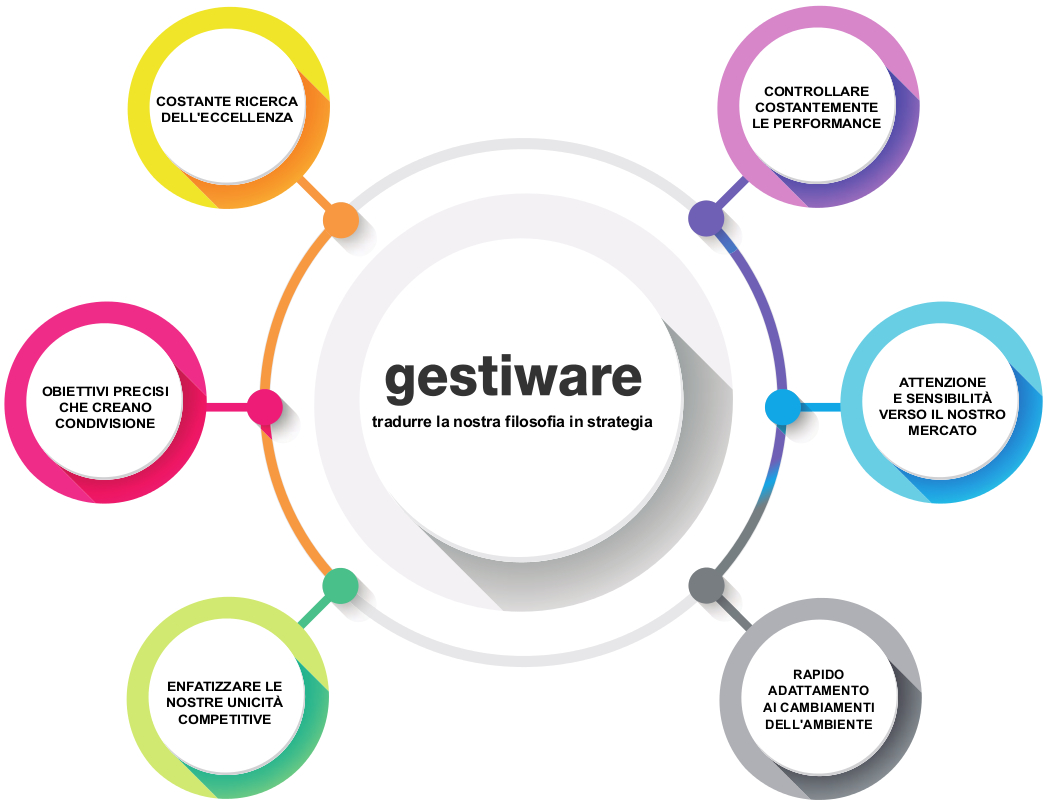
\includegraphics[width=1\columnwidth]{immagini/505-TEST4.jpg}
        \caption{Presentazione azienda}
    \end{figure}
    \newpage
\subsection{Servizi offerti}
    L'attività aziendale riguarda tre aree principali: 
    \begin{itemize}
        \item prodotti software;
        
        \item consulenze architetturali e organizzative;
        
        \item realizzazioni di progetti enterprise.
    \end{itemize}
    F12 è un software \emph{ERP}\glsfirstoccur completo in grado di supportare l'azienda in tutte le sue principali attività: amministrazione, flusso acquisti e vendite e supervisione della produzione.
    \\
    F12 unisce l'esperienza raccolta dai soci fondatori nel settore alle tecnologie e modalità operative odierne, garantendo stabilità e flessibilità nella gestione dei dati aziendali.
    \\
    Da una linea di sviluppo principale ed orientata ad un'azienda manifatturiera in
    generale, sono state derivate personalizzazioni specifiche per i vari settori produttivi, come ad esempio quello del mobile, chimico, servizi, cantieri eristica navale e da diporto, alimentare, cartotecnico, ecc.
    \\
    Oltre alle personalizzazioni orientate al settore produttivo, Gestiware ha dedicato un
    significativo periodo di tempo allo studio e realizzazione di interfacce di comunicazione fra F12 ed altri software di interesse aziendale. 
    \\
    Nell'ambito del sistema ERP, la ricerca si è focalizzata sul miglioramento delle tecniche
    tradizionali di gestione del magazzino e della produzione, offrendo un set di strumenti
    innovativi che riducono notevolmente i costi di gestione in questi ambiti, sia in termini
    monetari che computazionali.
    
\subsection{Vantaggi aziendali}
Per Gestiware S.r.l. i percorsi di tirocinio, sia universitari che per la scuola secondaria di secondo grado, sono fondamentali in quanto permettono all'azienda di entrare in contatto con ragazzi ed istituti con l'obiettivo di proporre un futuro impiego o collaborazione.

%**************************************************************
\section{Convenzioni tipografiche}
Nei paragrafi di questa sezione sono riportate le norme tipografiche adottate per la stesura del seguente testo. Lo scopo di tali norme è quello di produrre un documento rigorosamente formale e coerente.
\\
\\
\textbf{Glossario.} Per la prima occorrenza dei termini riportati nel glossario, situato alla fine del presente documento, viene utilizzata la seguente nomenclatura: \emph{parola}\glsfirstoccur;
\\
\\
\textbf{Elenchi puntati.} Gli elenchi puntati servono ad esprimere un concetto in modo sintetico e strutturato, evitando di utilizzare uno stile troppo narrativo, che mal si adatta in documenti di tipo tecnico-informativo. \newline
Ogni voce nell'elenco puntato inizia con la lettera minuscola (tranne dove è necessario la lettera maiuscola, per esempio con nomi di attività) e finisce con un punto e virgola, ad eccezione dell'ultima, che si conclude con un punto.\newline
Se l'elenco ha l'obiettivo di descrivere punti salienti, allora il nome del termine va scritto in grassetto, con la prima lettera maiuscola e se è presente la relativa descrizione va inserita dopo i due punti. 
\\
\\
\textbf{Stile del testo}
\begin{itemize}
    \item \textbf{Grassetto:} verrà usato per titoli e per elementi che riassumono il contenuto in un elenco puntato, come in questo caso con la parola "Grassetto";
    
    \item \textbf{Corsivo:} verrà usato per citazioni, abbreviazioni e termini rilevanti da evidenziare;
    
    \item \textbf{Maiuscolo:} verrà usato per acronimi o per nomi che lo richiedono.
    
    \item \textbf{Virgolette:} verranno usate per citazioni, riferimenti a frasi o parole riportate precedentemente nel testo, nomi di documenti, voci di menù o voci di pulsanti da premere.
\end{itemize}




%**************************************************************
\section{Struttura del documento}

\begin{description}
    \item Il secondo capitolo, {\hyperref[cap:descrizione-stage]{Descrizione dello stage}}, riporta una breve descrizione dei possibili rischi, le modalità di svolgimento e la pianificazione dell'attività di stage svolta. Inoltre è riportata, a grandi linee, la richiesta dell'azienda proponente seguita dalla soluzione da me progettata per far fronte ad essa.
    
    \item Il terzo capitolo, {\hyperref[cap:protocollazione]{Protocollazione}}, approfondisce questa tematica fornendone una definizione, illustrandone la metodologia di registrazione di un protocollo e illustrandone la necessità di configurazione dei flussi applicativi.
    
    \item Il quarto capitolo, {\hyperref[cap:gestione-documentale]{Gestione documentale}}, approfondisce e illustra il software "F12 Documentale" fornitomi da Gestiware S.r.l. per una facile ed efficiente gestione dei documenti caricati attraverso il prodotto da me realizzato.
    
    \item Il quinto capitolo, {\hyperref[cap:progettazione-codifica]{Progettazione e codifica}}, approfondisce ogni singolo aspetto di queste due attività fondamentali da me svolte durante lo stage.
    
    \item Il sesto capitolo, {\hyperref[cap:verifica-validazione]{Verifica e validazione}}, descrive il lavoro svolto per quanto riguarda le attività di verifica e di validazione. 
    
    \item Il settimo capitolo, {\hyperref[cap:conclusioni]{Conclusioni}}, contiene un'analisi riassuntiva degli obiettivi raggiunti, delle conoscenze acquisite e le conclusioni sull'attività svolta.
\end{description}